\chapter{Einführung}
\label{sec:intro}
	%\setcounter{page}{1}
	
	Im Laufe der Zeit werden immer mehr Prozesse digitalisiert bzw. 
	automatisiert - sei es in der Industrie, im zwischenmenschlichen 
	Bereich oder auch im Privathaushalt. Immer mehr Aufgabengebiete sollen vom 
	Menschen auf die Maschine übergehen, so auch der Vorgang des Sehens oder 
	auch des Erkennens von bestimmten Mustern. Dies ist für Industriebetriebe 
	insofern interessant, da es beispielsweise eine automatisierte 
	Identifizierung von Bauteilen anhand eines darauf angebrachten 
	Zeichencodes ermöglicht. Abbildung \ref{fig:example-code} zeigt 
	exemplarisch einen derartigen Code:
	\begin{figure}[h]
		\centering
		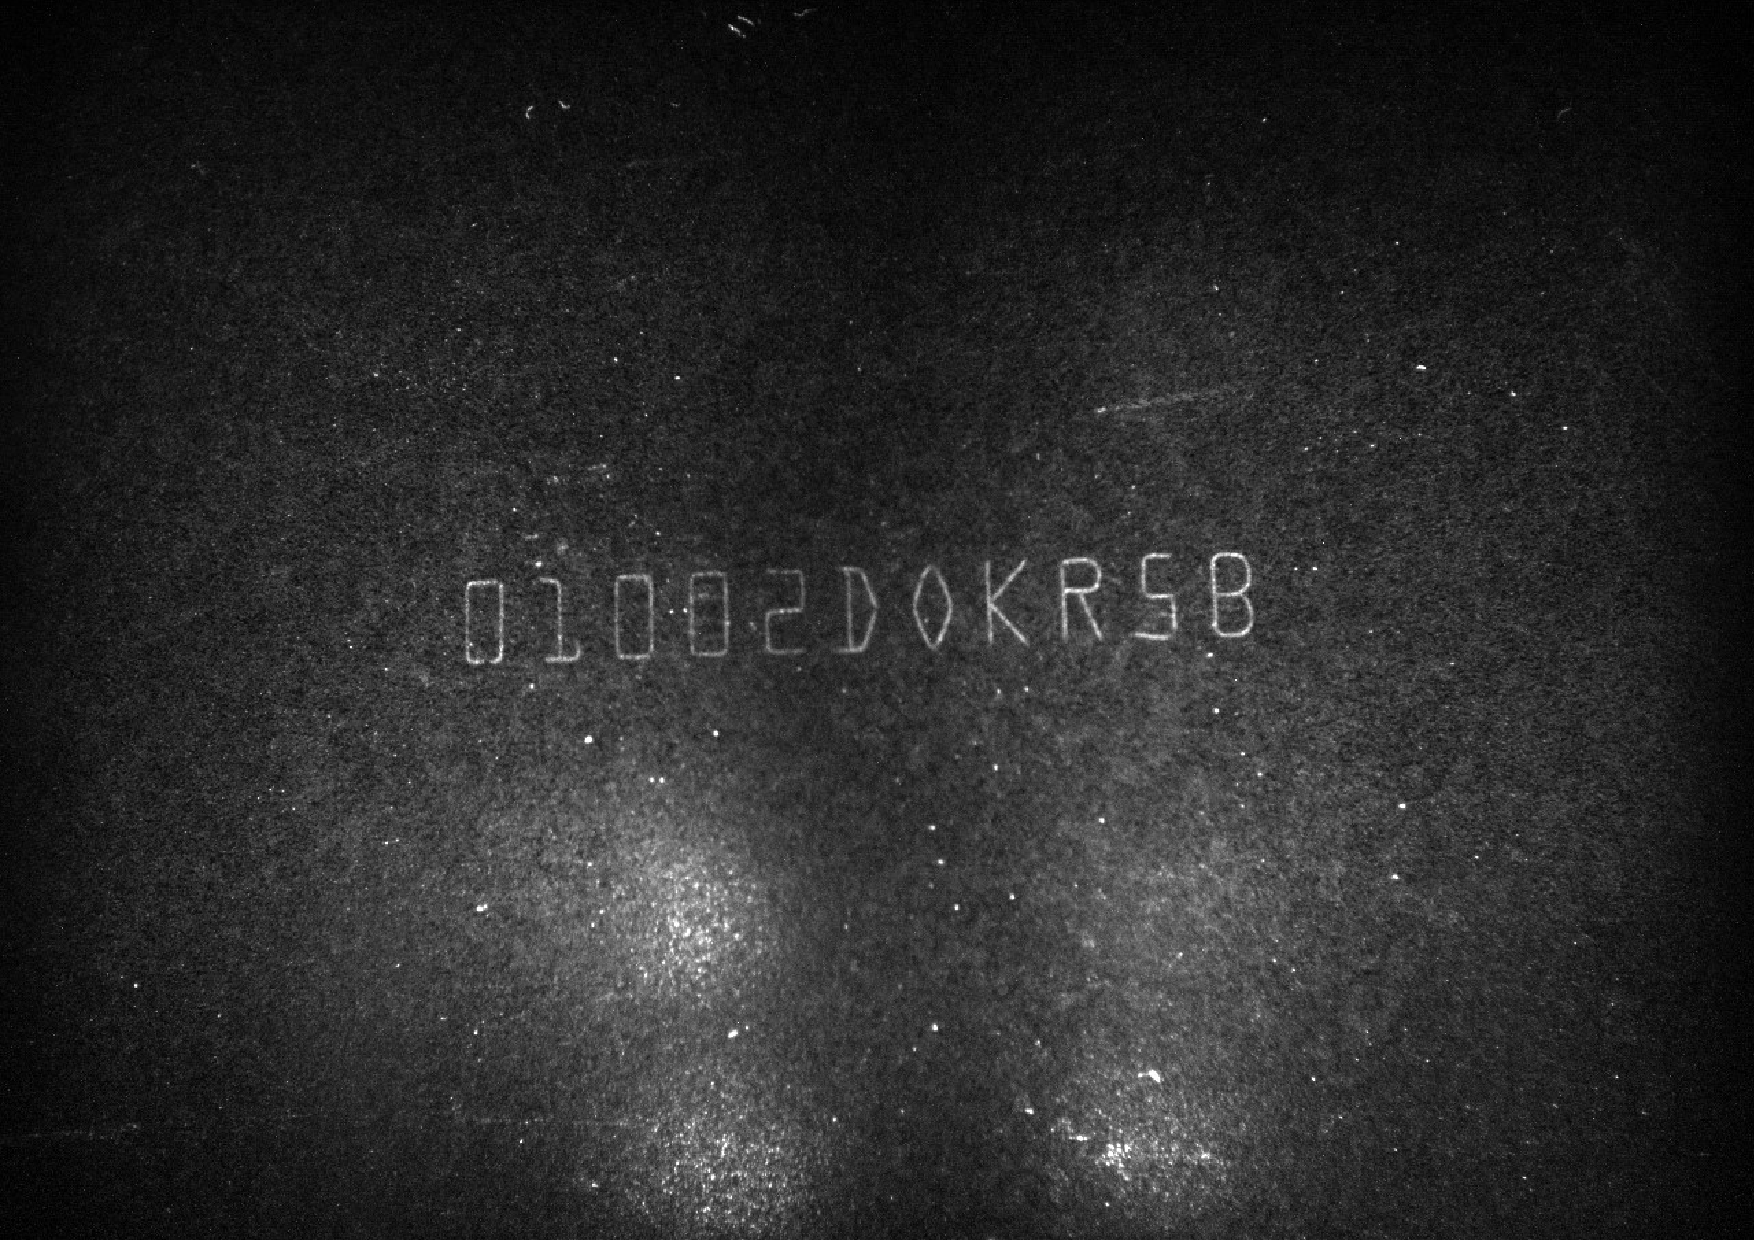
\includegraphics[width=\linewidth]{beispielcode}
		\caption{Eingravierter Code auf metallischem Bauteil}
		\label{fig:example-code}
	\end{figure}

	Einen solchen Code maschinell zu erkennen - ein Problem aus dem Fachgebiet 
	der \textit{\gls{ocr}}, ist keineswegs eine 
	triviale Aufgabe, wie in Kapitel \ref{sec:prob} herausgestellt wird. Bis 
	heute wurde dieses Problem nicht in einer Weise gelöst, die eine 100\% 
	Erfolgsquote in für die freie Wirtschaft praktikabler Zeit verspricht. Auf 
	der Suche nach einer zufriedenstellenden Lösung müssen unter anderem durch 
	Experimente mit unterschiedlichen Methoden Erkenntnisse gewonnen werden. 
	Hierzu soll im Übrigen auch diese vorliegende Arbeit einen Beitrag leisten, 
	indem sie untersucht, inwieweit ein ausgewähltes Verfahren aus der Gruppe 
	der \textit{evolutionären Methoden} dafür geeignet ist, einen wichtigen 
	Schritt innerhalb der \gls{ocr} zu realisieren. \\
	
	Dabei ist die folgende Struktur vorgesehen: \\
	In Kapitel \ref{sec:prob} werden die Hintergründe bzw. die grundlegende 
	Motivation aus der Bildverarbeitung - spezifischer ausgedrückt, aus der 
	\gls{ocr} - hinter dieser Arbeit beleuchtet.\\
	Kapitel \ref{sec:sol} formuliert konkret die Aufgabenstellung und zeigt Ansätze 
	zur Lösung dieser sowie die Umsetzung in Form von Programmcode auf.\\
	Daraufhin werden in Kapitel \ref{sec:results} die Ergebnisse aus der 
	Umsetzung der in Kapitel \ref{sec:sol} vorgestellten Ideen und eine 
	Interpretation der Resultate präsentiert.\\
	Abgerundet wird dieses Erzeugnis durch eine abschließende Bewertung sowie einen Ausblick auf die künftige Verwendung der in Kapitel \ref{sec:sol} erarbeiteten Implementierung.
